%%
%% This is file `sample-sigconf-authordraft.tex',
%% generated with the docstrip utility.
%%
%% The original source files were:
%%
%% samples.dtx  (with options: `all,proceedings,bibtex,authordraft')
%% 
%% IMPORTANT NOTICE:
%% 
%% For the copyright see the source file.
%% 
%% Any modified versions of this file must be renamed
%% with new filenames distinct from sample-sigconf-authordraft.tex.
%% 
%% For distribution of the original source see the terms
%% for copying and modification in the file samples.dtx.
%% 
%% This generated file may be distributed as long as the
%% original source files, as listed above, are part of the
%% same distribution. (The sources need not necessarily be
%% in the same archive or directory.)
%%
%%
%% Commands for TeXCount
%TC:macro \cite [option:text,text]
%TC:macro \citep [option:text,text]
%TC:macro \citet [option:text,text]
%TC:envir table 0 1
%TC:envir table* 0 1
%TC:envir tabular [ignore] word
%TC:envir displaymath 0 word
%TC:envir math 0 word
%TC:envir comment 0 0
%%
%%
%% The first command in your LaTeX source must be the \documentclass
%% command.
%%
%% For submission and review of your manuscript please change the
%% command to \documentclass[manuscript, screen, review]{acmart}.
%%
%% When submitting camera ready or to TAPS, please change the command
%% to \documentclass[sigconf]{acmart} or whichever template is required
%% for your publication.
%%
%%
\documentclass[sigconf]{acmart}
\usepackage{hyperref}
%%\usepackage{indentfirst}

%%
%% \BibTeX command to typeset BibTeX logo in the docs
\AtBeginDocument{%
  \providecommand\BibTeX{{%
    Bib\TeX}}}

%% Rights management information.  This information is sent to you
%% when you complete the rights form.  These commands have SAMPLE
%% values in them; it is your responsibility as an author to replace
%% the commands and values with those provided to you when you
%% complete the rights form.
\setcopyright{acmlicensed}
\copyrightyear{2018}
\acmYear{2018}
\acmDOI{XXXXXXX.XXXXXXX}

%% These commands are for a PROCEEDINGS abstract or paper.
\acmConference[PRI - G51]{Make sure to enter the correct
  conference title from your rights confirmation email}{October 13, 2024}{Porto, PT}
%%
%%  Uncomment \acmBooktitle if the title of the proceedings is different
%%  from ``Proceedings of ...''!
%%
%%\acmBooktitle{Woodstock '18: ACM Symposium on Neural Gaze Detection,
%%  June 03--05, 2018, Woodstock, NY}
\acmISBN{978-1-4503-XXXX-X/18/06}


%%
%% Submission ID.
%% Use this when submitting an article to a sponsored event. You'll
%% receive a unique submission ID from the organizers
%% of the event, and this ID should be used as the parameter to this command.
%%\acmSubmissionID{123-A56-BU3}

%%
%% For managing citations, it is recommended to use bibliography
%% files in BibTeX format.
%%
%% You can then either use BibTeX with the ACM-Reference-Format style,
%% or BibLaTeX with the acmnumeric or acmauthoryear sytles, that include
%% support for advanced citation of software artefact from the
%% biblatex-software package, also separately available on CTAN.
%%
%% Look at the sample-*-biblatex.tex files for templates showcasing
%% the biblatex styles.
%%

%%
%% The majority of ACM publications use numbered citations and
%% references.  The command \citestyle{authoryear} switches to the
%% "author year" style.
%%
%% If you are preparing content for an event
%% sponsored by ACM SIGGRAPH, you must use the "author year" style of
%% citations and references.
%% Uncommenting
%% the next command will enable that style.
%%\citestyle{acmauthoryear}


%%
%% end of the preamble, start of the body of the document source.
\begin{document}

%%
%% The "title" command has an optional parameter,
%% allowing the author to define a "short title" to be used in page headers.
\title{PRIMED: A Medicine Search System}

%%
%% The "author" command and its associated commands are used to define
%% the authors and their affiliations.
%% Of note is the shared affiliation of the first two authors, and the
%% "authornote" and "authornotemark" commands
%% used to denote shared contribution to the research.
\author{Pedro Simões}
\email{up202403063@up.pt}
\affiliation{%
  \institution{Faculdade de Engenharia da Universidade do Porto}
  \city{Porto}
  \country{Portugal}
}

\author{Miguel Garrido}
\email{up202108889@up.pt}
\affiliation{%
	\institution{Faculdade de Engenharia da Universidade do Porto}
	\city{Porto}
	\country{Portugal}
}

\author{Emanuel Maia}
\email{up202107486@up.pt}
\affiliation{%
	\institution{Faculdade de Engenharia da Universidade do Porto}
	\city{Porto}
	\country{Portugal}
}

\author{Guilherme Martins}
\email{up202403106@up.pt}
\affiliation{%
	\institution{Faculdade de Engenharia da Universidade do Porto}
	\city{Porto}
	\country{Portugal}
}

%%
%% By default, the full list of authors will be used in the page
%% headers. Often, this list is too long, and will overlap
%% other information printed in the page headers. This command allows
%% the author to define a more concise list
%% of authors' names for this purpose.
\renewcommand{\shortauthors}{Pedro Simões, Miguel Garrido, Emanuel Maia and Guilherme Martins}

%%
%% The abstract is a short summary of the work to be presented in the
%% article.
\begin{abstract}
    Factors like the simultaneous aging and growth of the population, as well as a larger prevalence of health issues, have lead to a higher demand for medical solutions and associated information systems. In this context, the project tackles the issue of efficiently searching for information about medicines, the diseases they treat and potential side-effects, as well as the companies that produce them and feedback left by other patients.
    Therefore, this article's goal is to provide clear and extensive insights on the development of a search engine for the medicines themselves and other aforementioned associated information, by integrating previously prepared data collected from multiple sources and properly analysing it.
\end{abstract}

%%
%% The code below is generated by the tool at http://dl.acm.org/ccs.cfm.
%% Please copy and paste the code instead of the example below.
%%
\begin{CCSXML}
<ccs2012>
   <concept>
       <concept_id>10002951.10003317.10003325</concept_id>
       <concept_desc>Information systems~Information retrieval query processing</concept_desc>
       <concept_significance>100</concept_significance>
       </concept>
 </ccs2012>
\end{CCSXML}

\ccsdesc[100]{Information systems~Information retrieval query processing}

%%
%% Keywords. The author(s) should pick words that accurately describe
%% the work being presented. Separate the keywords with commas.
\keywords{Medicine, Treatments, Sickness, Pipeline, Data, Gathering, Scraping, Preparation, Search Engine}
%% A "teaser" image appears between the author and affiliation
%% information and the body of the document, and typically spans the
%% page.
\begin{teaserfigure}
  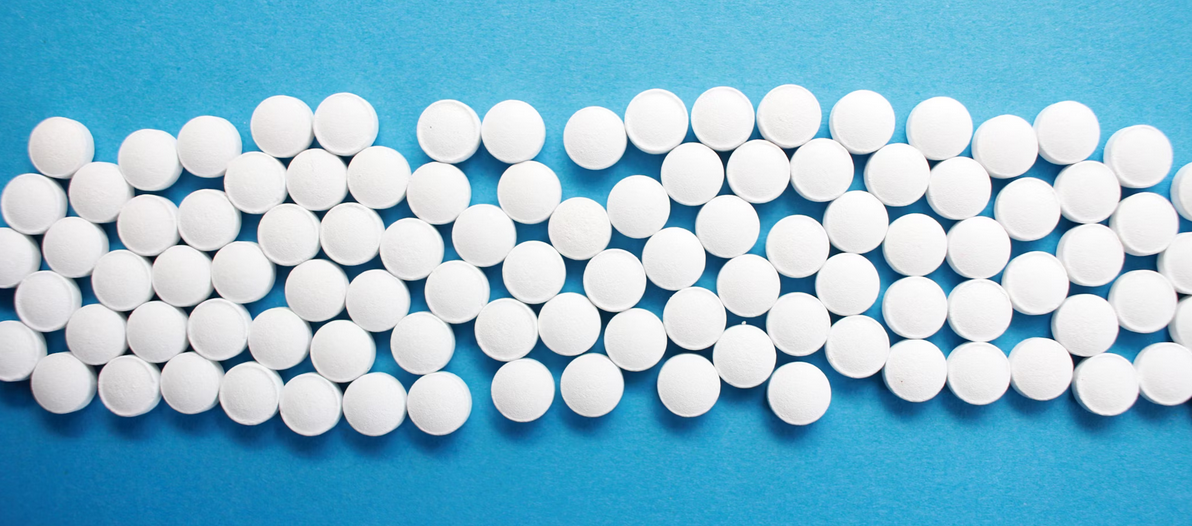
\includegraphics[width=\textwidth]{medicine.png}
  \caption{Figure 1: Medicine.}
  \Description{}
  \label{fig:teaser}
\end{teaserfigure}

\received{20 February 2007}
\received[revised]{12 March 2009}
\received[accepted]{5 June 2009}

%%
%% This command processes the author and affiliation and title
%% information and builds the first part of the formatted document.
\maketitle

\section{Introduction}
Nowadays, accurate and comprehensive medicine information plays a vital role in decision-making on the healthcare and investigation sectors. Having access to clean and relevant information is crucial to enhance the efficiency and safety of treatments.

The \textit{\textbf{PRIMED}} project aims to compile and organize such data so that it can be accessed in an easy and organized way. It provides insights that can be applied both in practical cases or simply in developing new health safety politics.

In this part of the project, data from various sources was collected, processed and analysed with the goal of creating a solid basis for a pharmaceutical system. The whole process is described in this document, from the choice of the theme itself up to the analysis of gathered data and its subsequent classification.

\section{Theme Selection}
The choice to focus on medicines as the central theme for this project stems from the critical role they play in modern healthcare. Medication is the primary tool for treating multiple health problems and conditions, making them an essential component in both public healthcare systems and individual patient care. The data surrounding these substances, such as active substances, applicable cases and clinical trials, offers valuable insights that can improve decision-making in medical practice and pharmaceutics.

\section{Data Collection}
This chapter outlines the data selection process and the methods utilized to gather it.

\subsection{Selection of Data}
One of the main challenges of the healthcare sector is ensuring that accurate and up-to-date information on medication is available to healthcare professionals. Given these needs, the selection of data to be collected was made:

\begin{itemize}
	\item {\texttt{Medicines}}: The main component of the data, consisting of medicines and their respective relevant, intrinsic information.
	\item {\texttt{Diseases}}: To complement the collected data, information on some diseases was collected so that it would be possible to get more information to allow for an easier medicine selection process.
	\item {\texttt{Pharmaceutical Companies}}: Some pharmaceutical companies are more trusted than others due to their credibility and higher quality products, which can impact the decision-making process.
	\item {\texttt{Reviews}}: It is important to know the success rate of the presented medicine and how the people who use it feel about it.
\end{itemize}

With this data, the aim is to provide the required information to the users.

\subsection{Gathering}

Finding data suitable for the project proved to be a challenge; not only did it have to be relevant and accurate, but it also had to meet some criteria in terms of quantity and quality. Therefore, the data had to be gathered from multiple sources using different methods - most of the data came from prepared datasets found on Kaggle\cite{kaggle}, while the rest came from scraping Wikipedia\cite{wikipedia}.

\subsubsection{Medicines}

The \textit{Medicines} dataset\cite{medicines_dataset}, retrieved from Kaggle, contains a list of pharmaceutical treatments and some relevant, mostly textual, information about the cases where it is used.

The present information on this dataset is:
\begin{itemize}
	\item {\texttt{Medicine Name}}: The name of the medicine.
	\item {\texttt{Composition}}: The active substance present in the medicine.
	\item {\texttt{Uses}}: A list of cases where the medicine is used (specific diseases, for example).
	\item {\texttt{Side Effects}}: Lists possible side effects resulting from the medicine's usage.
	\item {\texttt{Manufacturer}}: The name of the company responsible for producing the medicine.
	\item {\texttt{Reviews}}: Three additional columns containing the percentage of "Excellent", "Average" and "Poor" reviews for each medicine's treatment results.
\end{itemize}

This dataset possesses a {\textit{\textbf{CC0 1.0 Universal}}}\cite{cczero} license, which means the data is part of the public domain, allowing for the copying and modification of the data.

\subsubsection{Diseases}

This dataset was scraped from the tables of a Wikipedia page containing a list of autoimmune diseases\cite{diseases_dataset}; by gathering this data, the goal was to complement the previous dataset's "Uses" and "Side Effects" columns by collecting more information on this specific subset of diseases.

The information extracted from this dataset consists of:
\begin{itemize}
	\item {\texttt{Disease}}: The name of the disease.
	\item {\texttt{Primary Organ/Body Part Affected}}: Information on the organs or body parts affected by the disease.
	\item {\texttt{Autoantibodies}}: The antibodies associated with each specific disease.
	\item {\texttt{Acceptance as an Autoimmune Disease}}: Classification for each disease related to its acceptance as an autoimmune condition, based on the current scientific consensus and level of evidence supporting its autoimmune nature.
	\item {\texttt{Prevalence Rate (US)}}: The percentage of people or how many the disease affects in the US.
\end{itemize}

The gathered dataset contains about 110 lines of diseases, being available under the \textit{\textbf{Creative Commons Attribution-ShareAlike 4.0 International}}\cite{wikipedia_cc} license, which allows for the sharing and adaptation of the contents.

\subsubsection{Pharmaceutical Companies}

To complement the data on companies present in the \textit{Medicines} dataset, more data on pharmaceutical companies was gathered through another round Wikipedia scraping - this time from a page containing an extensive list of pharmaceutical companies\cite{companies_dataset}. Approximately 700 companies' names and founding dates were gathered, alongside a short description from each one's Wikipedia article.

The collected information follows this structure:
\begin{itemize}
	\item {\texttt{Company Name}}: The company's name.
	\item {\texttt{Year}}: The year the company was created and, if available, when the company was shut down.
	\item {\texttt{Description}}: A short description of each company, its values and some extra information.
\end{itemize}

This dataset falls under the same license as the previous \textit{Diseases} dataset (\textit{\textbf{Creative Commons Attribution-ShareAlike 4.0 International}}), as the data was collected in a similar way.

\subsubsection{Reviews}

Lastly, a dataset containing reviews for the collected medication data with more personal descriptions from users\cite{reviews_dataset} was retrieved from UC Irvine's Machine Learning Repository\cite{irvine}.

The data collected had the following structure:
\begin{itemize}
	\item {\texttt{Unique ID}}: The unique identification of the review.
	\item {\texttt{Drug Name}}: Name of the drug/treatment.
	\item {\texttt{Condition}}: The condition of the patient where it was used.
	\item {\texttt{Review}}: Written review of the experience of taking the drug.
	\item {\texttt{Rating}}: Number from 0-10 that expresses the quality of the drug.
    \item {\texttt{Date}}: Date of when the drug was taken.
    \item {\texttt{Useful Count}}: Similar to a "like" system, this showcases the number of people who found this review useful.
\end{itemize}

This dataset contains around 215000 entries and is covered by the \textit{\textbf{Attribution 4.0 International}}\cite{ccfour} license, which allows for the sharing and adaptation of the datasets for any purpose, provided that the appropriate credit is given.

\section{Pipeline Description}

As mentioned in section 3.2 of this report, \textit{\textbf{PRIMED}}'s data comes from various sources. Due to the often unstructured nature of this data, it is vital to have a streamlined and automated way of normalizing and processing all the information into similar formats, which is the main role of the data pipeline.

The pipeline consists of \texttt{Python} scripts utilizing libraries such as \texttt{pandas}, \texttt{unidecode}, \texttt{html}, \texttt{json} and \texttt{csv} with the crux of the data processing occurring on the \texttt{to{\textunderscore}json.py} script, which converts the \texttt{CSV} files into \texttt{JSON} format.

\subsection{Elimination of Null Values and Rows}

When processing data, another key aspect to consider is that not all data may be correct or even present. For this reason, before doing anything else with the \texttt{CSV} source files, the pipeline uses \texttt{pandas} \textit{dataframes} to check for and remove rows containing only null values, or rows in which key values, such as \texttt{Medicine Name}, for instance, aren't present.

\subsection{Text Normalization}

When scraping information from websites, it is important to make sure all the text is normalized. The data pipeline ensures, via \texttt{Python}'s \texttt{unidecode()} function, that the dataset only contains \texttt{ASCII} characters. This helps prevent future issues when searching the datasets for information.

Another character normalization problem resulting from the scraping process arises due to \texttt{HTML}'s nature - more specifically, escape codes used to represent special characters. To convert these codes into ASCII characters, the \texttt{unescape()} function from \texttt{Python}'s \texttt{html} module, wrapped inside a call to the previously mentioned \texttt{unidecode()} function, to convert the \texttt{Unicode} output into \texttt{ASCII}.

\subsection{Standardization of Formats}

For the best possible result, formats such as dates should be standardized; therefore, part of the pipeline deals with transforming this data into \texttt{yyyy-mm-dd} format, which makes the process of sorting and searching substantially easier. 

\subsection{Data Storage}

maybe? describe how data is stored? buwomp

\section{Conceptual Data Model}

Having finalized the data collection and the subsequent transformation and storage processes in the pipeline, a conceptual data model for the combined dataset was developed.

\begin{figure}[H]
  \centering
  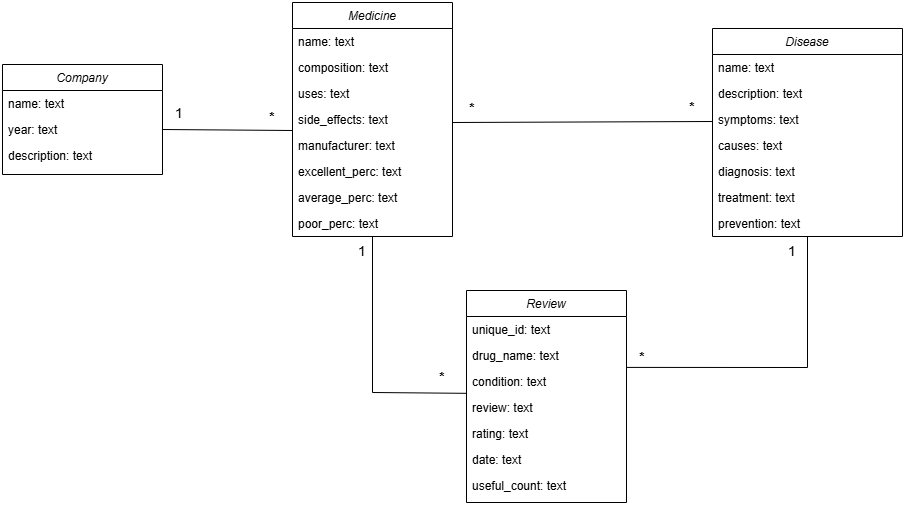
\includegraphics[width=\linewidth]{pri_uml_final.png}
  \caption{Conceptual Data Model}
  \Description{UML diagram for \textit{\textbf{PRIMED}}'s data}
  \label{fig:uml}
\end{figure}

Each medicine is associated with one and only one pharmaceutical company; a company, however, can produce multiple medicines. A single medicine can be linked to multiple diseases and reviews, though the reverse is true only for diseases - a disease can be associated to many medicines (and many reviews). A review, however, can only be associated with a single medicine and a single disease.

\section{Information Needs}

The information needs on this data can vary from the person using it. If the one who is using the tool is, for example, a doctor or pharmaceutical, the needs might be related to the compositions of medicine or cases where it was applied. If the user is an average person, he can be more interested in checking who made the medicine to check if it can be trusted or to check other user's reviews on that treatment/possible side effects to have a better understanding of what can happen to him.

Here is a list of possible information needs, explaining what kind of data on the is needed, why and for whom:
\begin{itemize}
	\item {\texttt{Medicine compositions}}: The composition of the treatment is important because some might even harm the patient so it is important to keep an eye out for that.
	\item {\texttt{Uses}}: Not every medicine has clear use cases, some might have a principal use but an also good side use that is not much common.
	\item {\texttt{Side effects}}: Clearly the users should be able to know the possible side effects of their treatment so that they can be prepared and informed of possible strange events.
	\item {\texttt{Manufacturer}}: Some people have preferential manufacturers who they trust more than others or can simply want to know more about the one they were prescribed.
	\item {\texttt{Reviews}}: For all possible types of users, the reviews are always important, both textual or not, they indicate other experiences. Sometimes peculiar cases are described there where the patients got rare effects from said treatment.
	\item {\texttt{Diseases' primary organs/autoantibodies}}: In some cases, experts might need to know how what part of the body or what are the antibodies that are affected by the diseases in order to prescribe the best solution.
	\item {\texttt{Prevalence rate}}: It can also be relevant to note how common certain disease when making the diagnosis of the patient or just for statistics.
\end{itemize}

Based one these needs we can answer some questions like: 
\begin{itemize}
	\item Which medicines can are more commonly used for certain conditions?
	\item How different manufacturers affect the treatment of specific diseases?
	\item How can certain health conditions be treated with the most effectiveness?
	\item With certain symptoms, what treatment should be applied?
	\item Are these effects normal after taking certain medication?
	\item What happened to other people who had the same treatment as me?
\end{itemize}

Lastly, as previously stated, people such as normal users, medicine experts and even investigators can take advantage from this type of information. From gaining awareness, to helping people with special needs on recovering.

\section{Dataset Characterization}

With regard to Dataset Characterization, the data from the pipeline was characterized. Graphs, tables and word clouds were created to make it easier to understand the structure of the data and the patterns that guide the recommendations in the system.

\subsection{Distribution of drug manufacturers}

Figure [3] shows the distribution of the main drug manufacturers, highlighting those with the largest share. The analysis of the graph allows us to understand the concentration of the companies production of medicines.

\subsection{Distribution of Reviews}

In figure [4], in the box plot, we can analyze the distribution of the percentages of “Excellent”, “Average” and “Poor” reviews for the drugs. The graph shows that, in the majority of cases, medicines tend to receive “Average” reviews, while the “Excellent” evaluation has greater variation.

\subsection{Reviews percentages by uses}

In this stacked bar chart, in figure [5] we can see the average percentage of reviews for different uses. Each bar represents a use, divided between “Excellent”, “Average” and “Poor” reviews. 

\subsection{Distribution of side effects}

In the figure[6] In This bar chart shows us the number of drugs that are used for the different side effects. Among the most commonly treated effects are nausea, headache and diarrhea, which have the highest number of associated medications. This data shows a clear picture of the side effects that arise most frequently, and the amount of medication used to treat them.

\subsection{Common Uses Word Cloud}

The word cloud shows in the figure [7] the most common uses of medicines. “Bacterial Infections” and ‘Hypertension’ are examples of uses that appear most prominently, indicating that these are the diseases most frequently treated with medicines in the dataset.

\subsection{Most Common Drug Compositions}

In figure [8], the pie chart shows the five most common drug combinations. The combination “Levocetirizine + Montelukast” is the most frequent, followed by other combinations such as “Luliconazole” and “Domperidone + Rabeprazole”. This visualization makes it easier to identify the most popular compositions for treating diseases.

\subsection{Years with the Most Companies Foundations}	

In the bar chart shows in figure [9], we can see the years in which the most pharmaceutical companies were founded. 2003 is the year in which the most companies were founded. This temporal analysis helps us to understand the periods of greatest growth in the pharmaceutical industry.

\section{Conclusions}

Having completed this phase of preparing and analyzing data on medicines, we can say that this milestone was very important for the development of our system. The work carried out to date has made it possible to transform an initial set of diverse and scattered data into a cohesive and structured base. By carrying out data cleansing and integration techniques, we have been able to maintain the quality of the information, while reducing inconsistencies and duplications. By providing clear information on medicine, PRIME offers users a useful source for consultation, helping them to make more informed and safer health decisions.

\section{Annexes}

\begin{figure}[H]
	\centering
	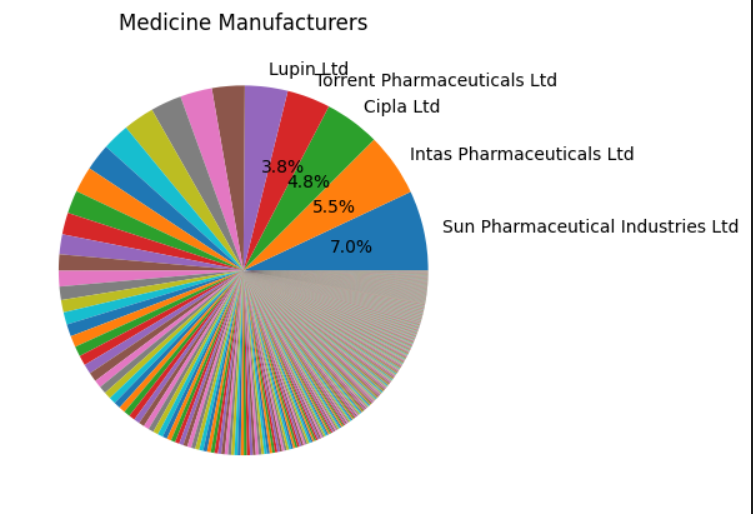
\includegraphics[width=\linewidth]{graphic1.png}
	\caption{Distribution of drug manufacturers}
	\Description{Dataset Characterization \textit{\textbf{PRIMED}}'s data}
	\label{fig:uml}
  \end{figure}

\begin{figure}[H]
	\centering
	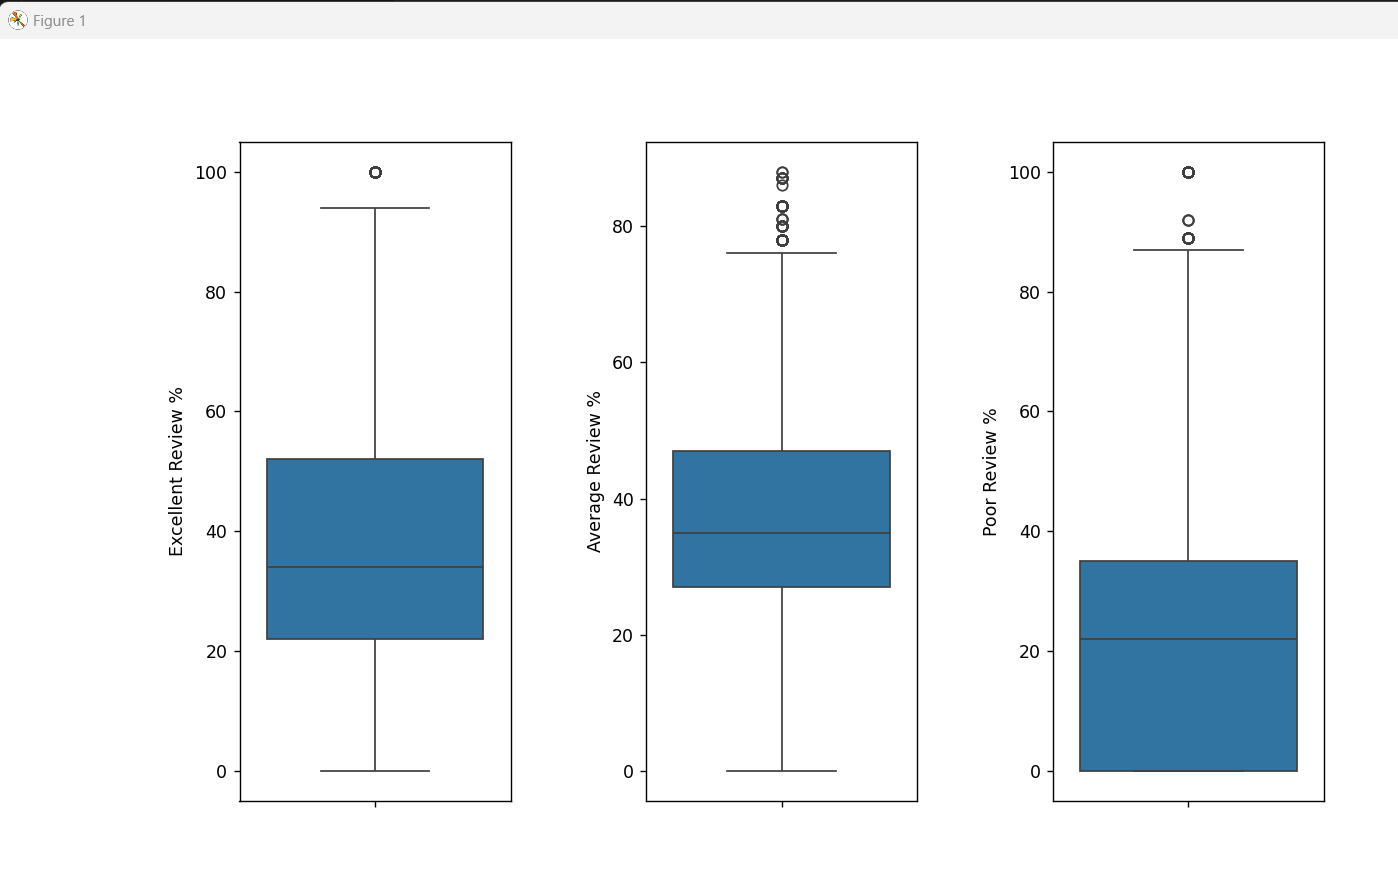
\includegraphics[width=\linewidth]{graphic2.png}
	\caption{Distribution of Reviews}
	\Description{Dataset Characterization \textit{\textbf{PRIMED}}'s data}
	\label{fig:uml}
  \end{figure}

\begin{figure}[H]
	\centering
	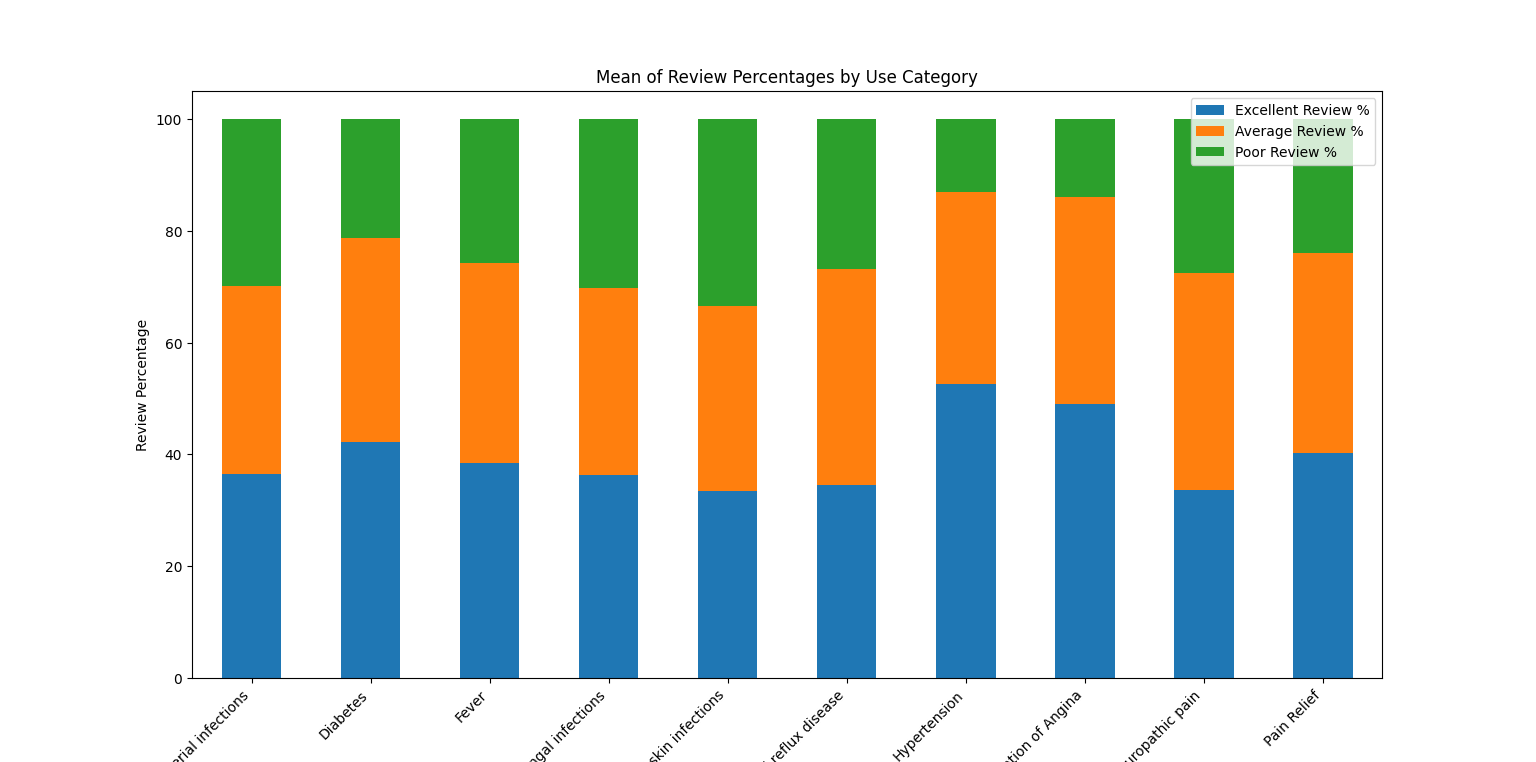
\includegraphics[width=\linewidth]{graphic3.png}
	\caption{Reviews percentages by uses}
	\Description{Dataset Characterization \textit{\textbf{PRIMED}}'s data}
	\label{fig:uml}
  \end{figure}

\begin{figure}[H]
	\centering
	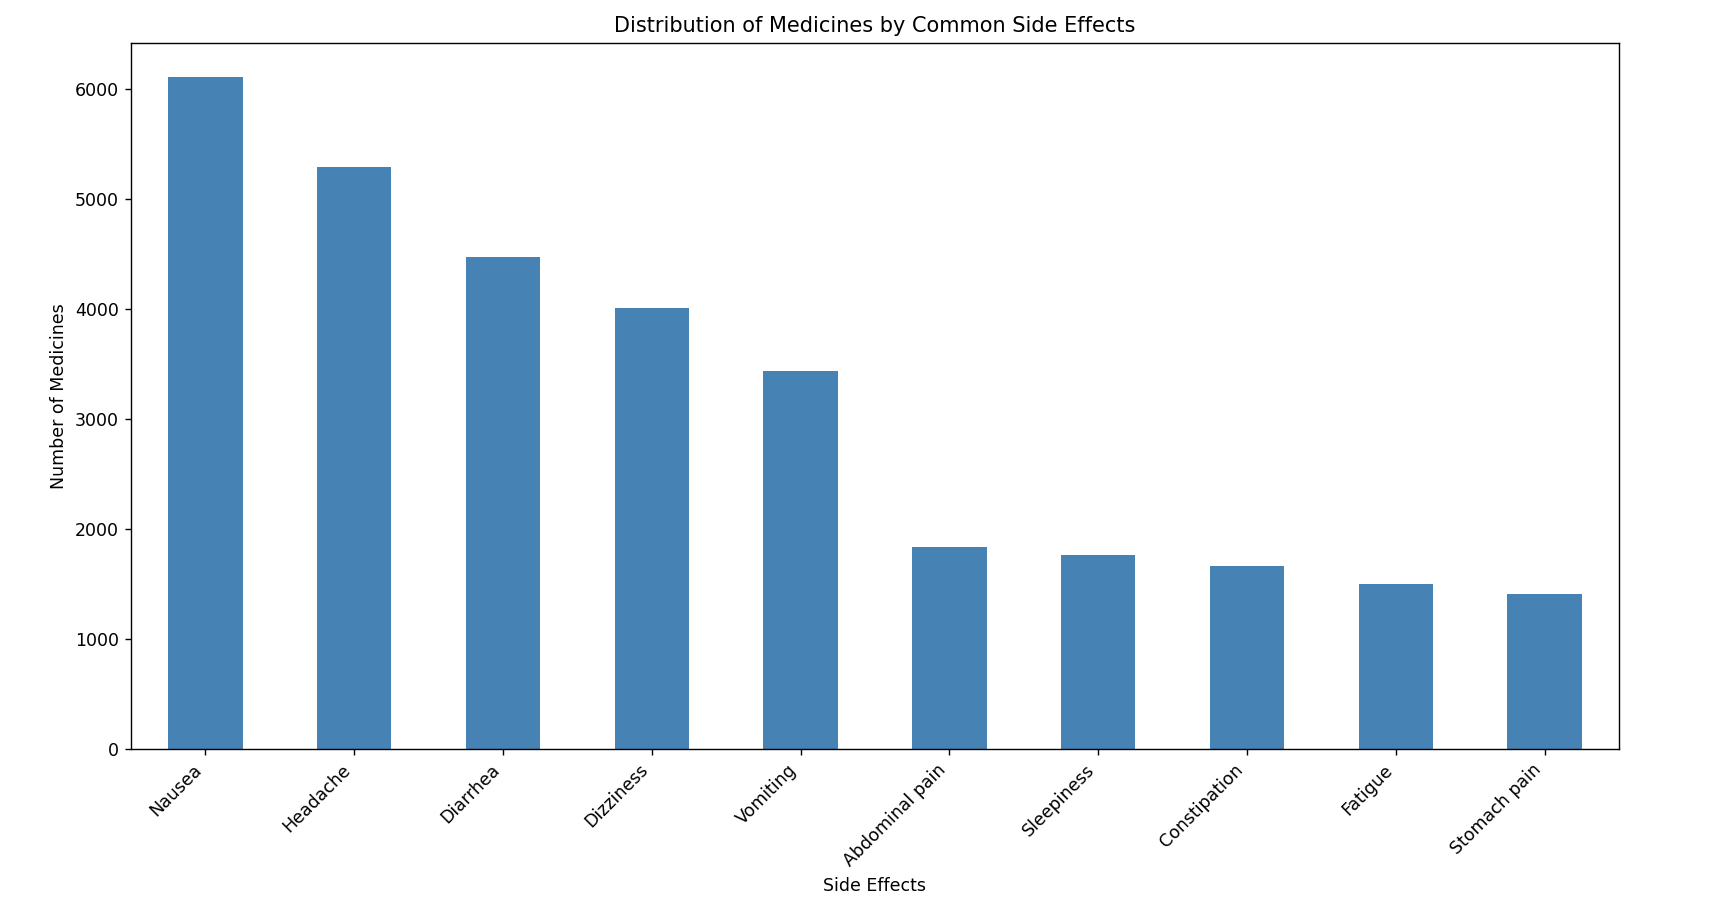
\includegraphics[width=\linewidth]{graphic4.png}
	\caption{Distribution of side effects}
	\Description{Dataset Characterization \textit{\textbf{PRIMED}}'s data}
	\label{fig:uml}
  \end{figure}

\begin{figure}[H]
	\centering
	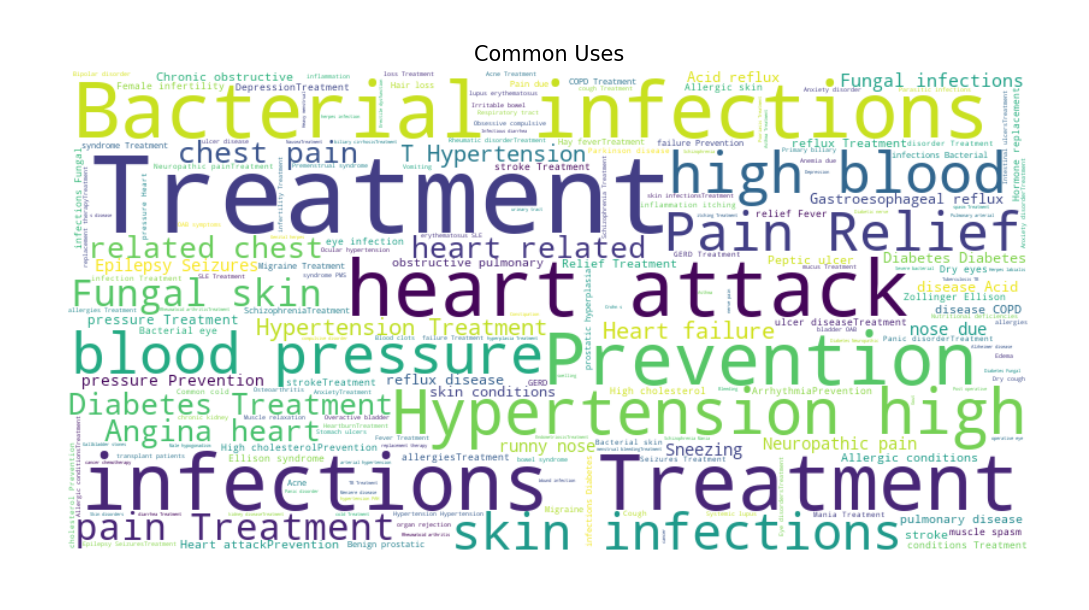
\includegraphics[width=\linewidth]{graphic5.png}
	\caption{Common Uses Word Cloud}
	\Description{Dataset Characterization \textit{\textbf{PRIMED}}'s data}
	\label{fig:uml}
  \end{figure} 

\begin{figure}[H]
	\centering
	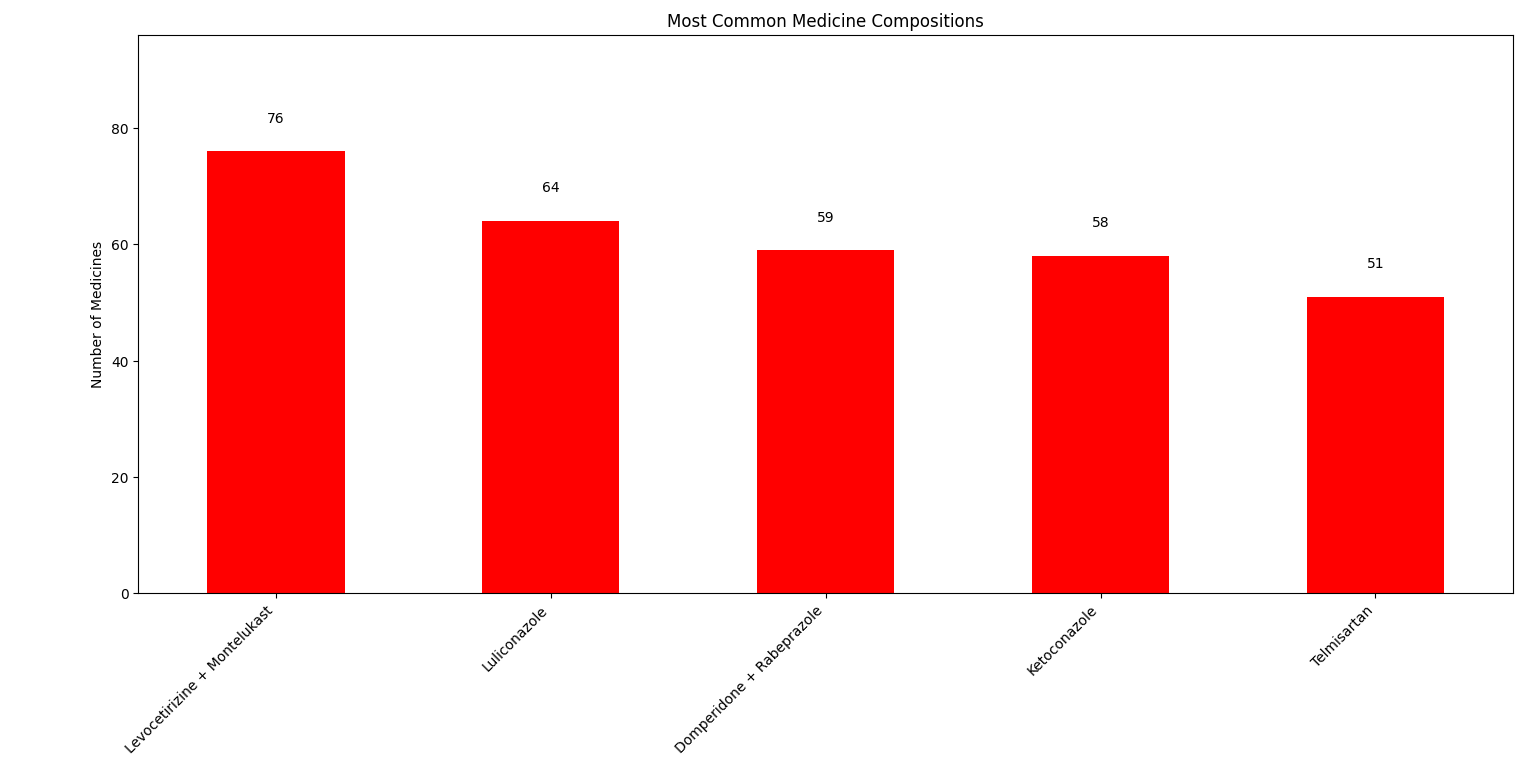
\includegraphics[width=\linewidth]{graphic6.png}
	\caption{Most Common Drug Compositions}
	\Description{Dataset Characterization \textit{\textbf{PRIMED}}'s data}
	\label{fig:uml}
  \end{figure}   

\begin{figure}[H]
	\centering
	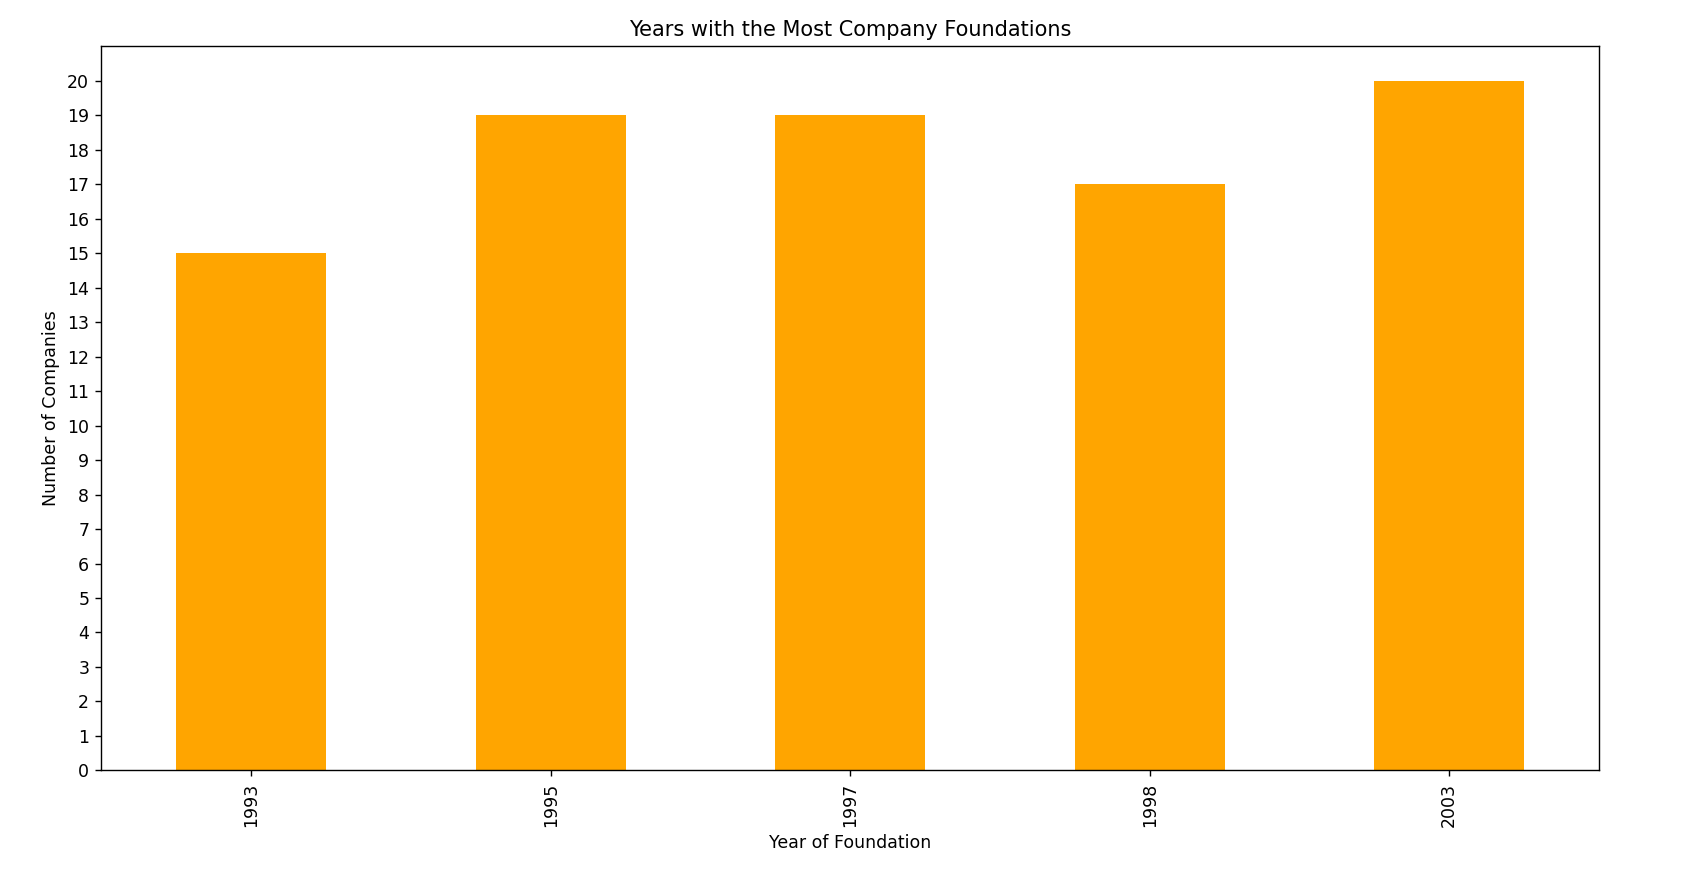
\includegraphics[width=\linewidth]{graphic7.png}
	\caption{Years with the Most Companies Foundations}
	\Description{Dataset Characterization \textit{\textbf{PRIMED}}'s data}
	\label{fig:uml}
  \end{figure}

%%
%% The next two lines define the bibliography style to be used, and
%% the bibliography file.
%%\bibliographystyle{ACM-Reference-Format}
\bibliographystyle{unsrt}
\bibliography{sample-base}


%%
%% If your work has an appendix, this is the place to put it.
\appendix

\section{Research Methods}

\subsection{Part One}

Lorem ipsum dolor sit amet, consectetur adipiscing elit. Morbi
malesuada, quam in pulvinar varius, metus nunc fermentum urna, id
sollicitudin purus odio sit amet enim. Aliquam ullamcorper eu ipsum
vel mollis. Curabitur quis dictum nisl. Phasellus vel semper risus, et
lacinia dolor. Integer ultricies commodo sem nec semper.

\subsection{Part Two}

Etiam commodo feugiat nisl pulvinar pellentesque. Etiam auctor sodales
ligula, non varius nibh pulvinar semper. Suspendisse nec lectus non
ipsum convallis congue hendrerit vitae sapien. Donec at laoreet
eros. Vivamus non purus placerat, scelerisque diam eu, cursus
ante. Etiam aliquam tortor auctor efficitur mattis.

\section{Online Resources}

Nam id fermentum dui. Suspendisse sagittis tortor a nulla mollis, in
pulvinar ex pretium. Sed interdum orci quis metus euismod, et sagittis
enim maximus. Vestibulum gravida massa ut felis suscipit
congue. Quisque mattis elit a risus ultrices commodo venenatis eget
dui. Etiam sagittis eleifend elementum.

Nam interdum magna at lectus dignissim, ac dignissim lorem
rhoncus. Maecenas eu arcu ac neque placerat aliquam. Nunc pulvinar
massa et mattis lacinia.

\end{document}
\endinput
%%
%% End of file `sample-sigconf-authordraft.tex'.
